\chapter{Design}
\label{chapter:Design}
%Overarching design in a top-down view: 
%-server/client design overall architecture, system model
%-describe file system, 
%-how protocol is peformed by the server
%-describe current functionality of the implementation. Handles protocol run, view-changes and checkpointing

%old version:-overall usage over different parameters, overaching stuff thats not the actual implementation of the algorithm, but the network layer to server to algorithm, how to run the algorithm/checkpointing/view changes.
%first draft!!!
This chapter present an overall summary of the PBFT application implemented. This includes a brief summary of the system model used for performing the PBFT algorithm. The structure of the application including a brief introduction to its file structure as well as describing the general design for performing the consensus algorithm. We will finally describe the current functionalities that are present in the current application. 
Remember to check previous sections for how I should mark names in the text!
\section{System Model}
\begin{figure}
	\centering
	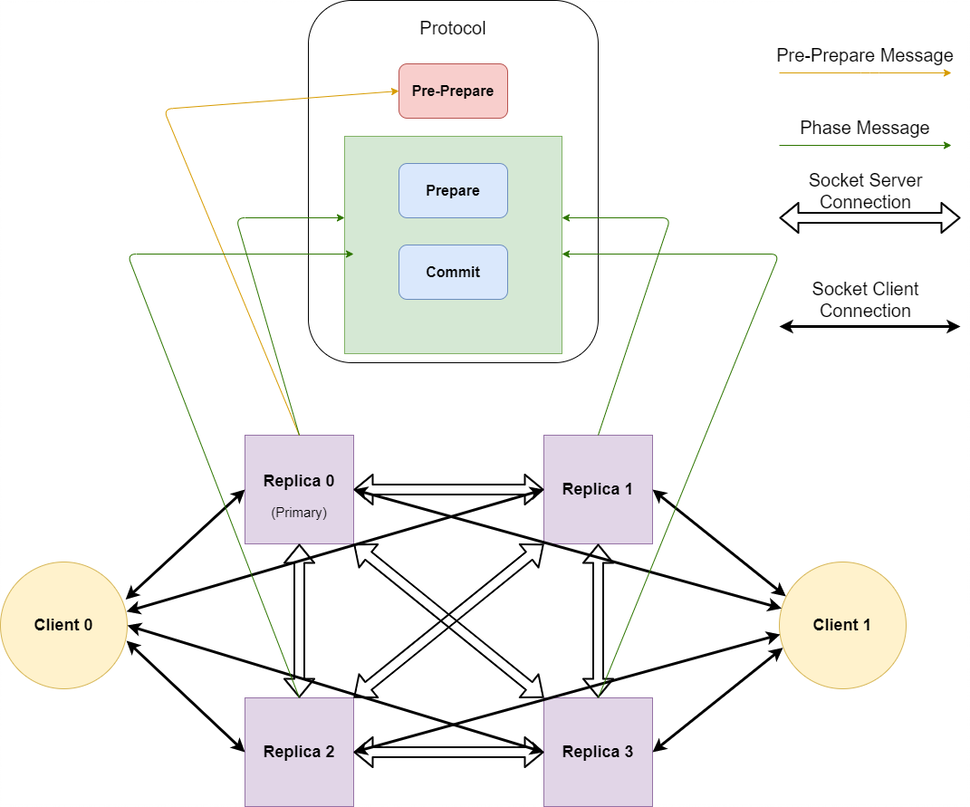
\includegraphics[width=\linewidth]{figures/meshnetwork}
	\caption{Overall architecture of the PBFT implementation networking}
	\label{fig:meshnetwork}
\end{figure}
The figure \autoref{fig:meshnetwork} shows the system model used for PBFT implementation. Generally our system model follows the same structure as the system model introduced in the PBFT chapter\autoref{sec:systemModel}. The system consist of four server implementations called \emph{replicas}, where the replica with the lowest identifier value is chosen as the primary. These four replicas are communicating over a mesh network using socket connections. This means each replica shares an unique network socket with each other replica in the PBFT network. In order to avoid creating multiple socket connections between replicas, the replica with the highest identifier is the one tasked with being the initiator when it comes to establishing a socket connection between other replicas. Meaning for instance that the primary replica, will not need to actively establish any connections to its fellow replicas. The primary will instead establish all of its socket connections by listening for any connections attempts on its local network address. The opposite scenario occurs for the replica with the highest identifier value, although the replica still listens for connections on its local network address, it is also responsible for establishing the connections with all the other replicas in the network with lower identifier values.

Even when the replicas have established connections, the replicas can not fully communicate with each other until they have exchanged public keys. This is required in order to verify messages sent by each replica using a digital signature. Public keys are exchanged in \emph{session messages}, which are messages that are automatically sent between parties once a socket connection has been established. If the public keys are for some reason not exchanged, than the replica will discard any message received from that host and thereafter terminate the connection. This also applies for clients. This current model is unfortunately not very secure, due to public keys being ephemeral and are intended to be replaced in the case of a crash occurring. Currently in this implementation, the private and public key pair for a replica are randomly created at the system start-up. Considering there is currently no way for the replicas to authenticate another replica after reboot, it will replace the key value pair currently in the register if a new session message with the same identifier value is received. This in turn means the system is susceptible to impersonation and spoofing attacks. Since the main goal of this thesis was more focused on the implementation of the PBFT workflow, this cryptographic system was deemed sufficient for simulating a network using digital signatures. However, it is important to be aware of this flaw in the system in order to avoid this issue in the future. %add how to fix this in future work.

The system performs the PBFT protocol by exchanging protocol messages over the mesh network until atleast three of the servers have finished all three protocol phases. In this implementation protocol messages are referred to as \emph{phase messages}. The PBFT protocol is trigger when the server receives a request from one of the connected client nodes. The primary is responsible for officially starting an instance of the PBFT protocol by multicasting a phase message of type pre-prepare. There are two important goals for the pre-prepare phase. The first is to make sure that the replicas have an agreement upon the ordering of the request. In other words, the replicas will perform the requests in the same order as the primary, which in turn means the request should have the same sequence numbers throughout the network. The second important goal is to determine whether or not the primary is fit to be leader. As mention in section \autoref{sec:view-change}, a view-change occurs when a leader no longer is eligible. In our application the view-changes are triggered by timeout which are set once a replica receives a client's request. If the primary takes too long in the pre-prepare phase, than the timeout will exceed and the other replicas will perform a view-change in order to change the primary replica. Although it would be useful to have timeouts in the commit phase in the instance where majority of servers are unable to properly finish the commit phase, it is currently not supported in our implementation due to how timeouts are handled inside the protocol workflow(should probably be moved elsewhere). The rest of the replicas will be the responsible party during the prepare phase by sending phase messages of type prepare, while every replica will participate in the commit phase using commit type phase messages. The last step of current PBFT implementation is to create a reply message and send it back to client responsible for the request. The details in regards to the PBFT workflow implementation will be discussed in the next chapter \autoref{chapter:Imp}.

\section{File structure}
In figure we \autoref{fig:filestruct} can see a short summary of the file system for our PBFT replica. The summary shows the root folders in our PBFT replica implementation. The summary also highlight some of the more important files, meaning files containing the most relevant code segments. 

\subsection{Folders}
To start of the PBFT implementations uses a lot of different types of message objects which are defined in their own seperate file. Therefore, all of the different message classes are stored within the \emph{Messages} folder. This includes interface that are shared among messages types. Similarly, there are several objects known as certificates which are used within this PBFT implementation and its class files and interfaces are stored within the \emph{Certificate folder}. Certificates are essentially records showing the status for the protocol states. For instance, the replica has a log which stores two certificates for each requests successfully handled by the PBFT protocol. These two certificates in the log will acts as proof for successful prepare and commit phases for that specific sequence number. 

The \emph{Helper} folder contains all the static functions used in the PBFT implementation that are not linked to any specific object instance. This includes functionality for serializing and deserializing messages objects with JSON~\cite{WEB:NewJSON}, cryptographic functions related to creating and validating digital signatures and files containing all the enum types used for this thesis. An enum is essentially a predefined dotnet class that has only constant values which are defined upon initialization and is really useful for classifying other objects~\cite{WEB:Enum}. In our PBFT implementation we have for instance used enums to categories the protocol phase a phase message belongs to. This allows the program to easily distinguish between pre-prepare, prepare and commit phase messages.  

The \emph{JSONFiles} contains the JSON files which contains the network addresses for each of the replicas in the system designated to their receptive identifier values. There exist two JSON files in this folder. The first file is used when running the implementation over multiple systems or over docker containers. The second file uses localhost addresses with different port numbers at is meant to be used when testing the system on a local device.

The PBFT replica implementation uses Cleipnir to persist important parts of the code in order for servers to easily be able to reconnect to the system. As discussed in chapter \autoref{chapter:Cleipnir}, Cleipnir has several different engine types which can be used to serialize and store the applications data. In our PBFT replica implementation, we have decided to use the \emph{Simple File Storage} engine. The \emph{Storage} folder will contain the .txt files in which Cleipnir stores its data in. Since there are several instances of replicas in the PBFT network, the name of the .txt file used to store the application data will follow the structure "PBFTStorage" with the replicas identifier value at the end of the name.

The \emph{Replica} folder contains code which are directly related to the server or code which are directly related to the protocol. The \emph{Replica} folder has two sub folders in order to easier distinguish between the files. The subfolder \emph{Network} contains code related to networking part. This includes the creation of sockets and functions for properly handling the data received from the socket by the TCP network protocol. 
The \emph{Protocol} sub folder contains code which are directly related to the protocol execution. This folder contains code related to the main workflow of the PBFT algorithm. In addition, code for handling the reactive execution for view-change and checkpointing can also be found in this folder.
The other files in the \emph{Replica} folder contains code that helps the replica run properly, including code which are used to help communication between server side and protocol workflow run inside Cleipnir.
The \emph{Storage} 

\subsection{Files}
The \emph{App.cs} file contains the code which starts all the processes needed in the PBFT replica. This includes code for starting Cleipnir, creating a server instance and starting the protocol handlers. This file also includes the main application state, which in this implementation is simply a list of operations theoretically performed by the system.

The \emph{Server.cs} file is by far the largest. This is due to the \emph{Server.cs} file being the bridge linking the network layer, responsible for sending and receiving messages properly, to the active protocol which requires the result of said messages. In addition to in general being responsible for most of the replica server side operations. 

The \emph{Workflow.cs} file is where the code for normal protocol workflow is stored, as well as where the code for performing the view-change protocol is stored. We will introduce the workflow found in this file in chapter \autoref{chapter:Imp}
%\newpage
\begin{wrapfigure}{r}{0.45\linewidth}
\centering
%\vspace{15pt}
%\rule{0.9\linewidth}{0.75\linewidth}
% ,scale=0.8, every node/.style={scale=0.8}
\tikzstyle{every node}=[draw=black,thick,anchor=west]
    \begin{tikzpicture}[%
      grow via three points={one child at (0.5,-0.7) and
      two children at (0.5,-0.7) and (0.5,-1.4)},
      edge from parent path={(\tikzparentnode.south) |- (\tikzchildnode.west)}]
      \node {PBFT}
        child { node {App.cs}}
        child { node {Certificates}
        	child {node {...}}
        	}	
        child [missing] {}
        child { node {Messages}
        	child {node {...}}
        	}
        child [missing] {}
        child { node {Helper}
        	child {node {...}}
        	}
        child [missing] {}
        child { node {JSONFiles}
        	child {node {serverInfo.json}}
        	child {node {testServerInfo.json}}
        	}
        child [missing] {}
        child [missing] {}
        child { node {Storage}
        	child {node {...}}
        }
        child [missing] {}
        child { node {Replica}
          child { node {Server.cs}}
          child { node {Network}
          	child {node {...}}
        	}
        }
        child [missing] {
          child { node {Protocol}
          child { node {Workflow.cs}}
          child { node {...}}
        	}
        };
\end{tikzpicture}
    \caption{Summary of the file architecture for the PBFT implementation}
    \label{fig:filestruct}
    \vspace{40pt}
\end{wrapfigure}

\begin{figure}[H]
	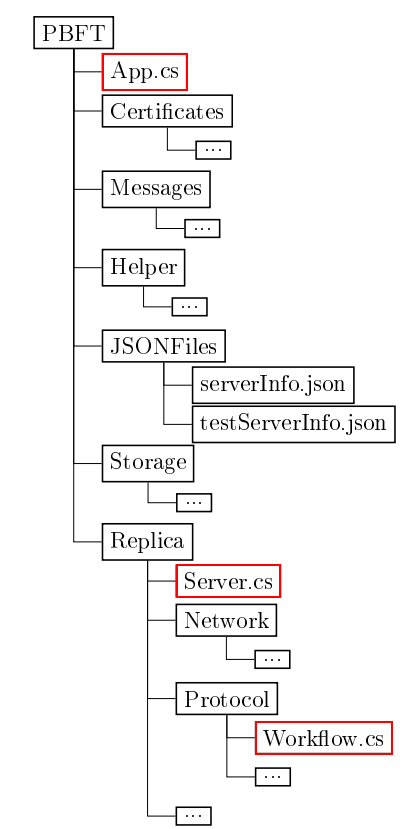
\includegraphics[width=0.45\linewidth]{figures/filestructtest}
	\caption{Summary of the file architecture for the PBFT implementation}
    \label{fig:filestruct}
\end{figure}

\newpage

\section{Server and protocol interaction}
%This will be a very large part, just need to figure out how to structure it.
Before we can introduce the main PBFT implementation workflow, it is first important to introduce the relationship between the server side and the protocol workflow. The server side is responsible for handling any received messages from the mesh network and properly emit the message to its proper reactive operator waiting for new messages to arrive. There are a few exceptions to this rule, case in point if the message the message is needed for server-side rather than the PBFT protocol, the message is used directly by the server and no emits are made. An example of this being session messages. Meanwhile the protocol itself is only responsible for performing the PBFT phase steps sequentially for any request received from the clients. Therefore, the primary relationship between the server side and the PBFT protocol implementation is simply that the server will emit any messages it receives from the network layer and then emit these messages to the PBFT protocol so that it can continue on with the workflow. As it is required for the PBFT protocol to multicast protocol messages during its workflow, the PBFT implementation also has a direct reference to the server, meaning it can easily send any messages it needs to the server in order for the server to multicast any messages out of its active sockets. This interaction may seem simple, however there is one aspect of there relationship that can be difficult. 

As mention in chapter \autoref{chapter:Cleipnir}, Cleipnir is a framework which main goal is to help create persistent consensus algorithms. We already discussed how easy it   
In Figure \autoref{fig:PersistencyEphemeral} parts of the PBFT implementation being divided into persistent parts and ephemeral parts. 


\begin{figure}[h]
	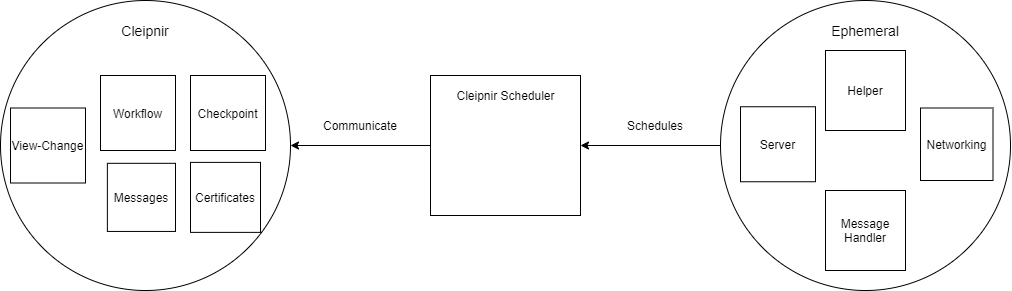
\includegraphics[width=\linewidth]{figures/CleipnirStructurever1}
	\caption{Application divided into persistent parts and ephermeral parts and how they interact}
	\label{fig:PersistencyEphemeral}
\end{figure}

\begin{figure}[h]
	\centering
	\lstset{style=sharpc}
	\begin{lstlisting}[label = code:schedulerEmit, caption= Example of server and protocol interaction using Cleipnir scheduler, captionpos=b, basicstyle=\scriptsize]
	public void EmitPhaseMessageLocally(PhaseMessage mes)
        {
            Console.WriteLine("Emitting Phase Locally!");
            if (ProtocolActive)
            {
                _scheduler.Schedule(() =>
                {
                    Subjects.ProtocolSubject.Emit(mes);
                });    
            }
        }
	\end{lstlisting}
\end{figure}